% % include the figures path relative to the master file
 \graphicspath{ {./content/experiment/figures/} }

\section{Experiments and Validation}
\label{sec:exp} \label{sec:exp:datasets}
An experimental suit is designed to test the influence of the different blocks composing our framework, using different datasets (see Table~\ref{tab:experiment_summary}).
T%o evaluate the effects and influence of the different blocks composing our framework, an experimentation suit has been designed to test different configuration parameters, which are evaluated using different datasets (see Table.~\ref{tab:experiment_summary}).
%The rest of this section details the design decisions that are consistent across all the experimentation, while subsections report different experiments.
The rest of this section details the common configuration parameters across all the experiments, while the following subsections focus on the specific aim of each experiment.

Unless stated otherwise, all the experiments are run using our own dataset alone, SERI.
Only for the sake of comparison, \emph{Experiment \#1} is performed on the public Duke dataset.
%SERI and Duke dataset details are reported in \ref{sec:exp:dataset:seri} and \ref{sec:exp:dataset:duke} respectively.
Acquisition details regarding SERI and Duke datasets are reported in Sect.\,\ref{sec:exp:dataset:seri} and Sect.\,\ref{sec:exp:dataset:duke}, respectively.

For all the experiments, \ac{lbp} and \ac{lbptop} features are extracted for different sampling points of 8, 16, and 24 for radius of 1, 2, and 3, respectively.
As previously mentioned, the \emph{local}- and \emph{global}-mapping strategies are used.
The partitioning for \emph{local}-mapping is set to ($7 \times 7$) patch for 2D \ac{lbp} and ($ 7 \times 7 \times 7$) sub-volume for \ac{lbptop}.
%where for \emph{local} mapping, we consider a ($7 \times 7$) \acf{sw} for 2D \ac{lbp} and ($ 7 \times 7 \times 7$) sub-volume for \ac{lbptop}.

All the experiments are evaluated using \ac{lopocv} strategy.
At each round, a pair \ac{dme}-normal volume is selected for testing while the remaining volumes are used for training.
The use of this method implies that no variance in terms of \acf{se} and \acf{sp} can be reported.
Despite this limitation, \ac{lopocv} has been employed due to the small size of the dataset.

All the experiments are evaluated in terms of \ac{se} and \ac{sp}, which are statistics driven from the confusion matrix (see Fig.\,\ref{fig:CM}) as stated in Eq.\,\ref{eq:sesp}.
The \ac{se} evaluates the performance of the classifier with respect to the positive class, while the \ac{sp} evaluate its performance with respect to negative class.
\begin{align}
 \ac{se}  = \frac{TP}{TP+FN} \qquad \ac{sp} = \frac{TN}{TN+FP}
 \label{eq:sesp}
\end{align}

Among all, one experiment is carried out using \ac{acc} and \ac{f1} as formulated in Eq.\,\ref{eq:accf1}.
\ac{acc} is used to have an overall sense of the classifier performance, and \ac{f1} is used to see the trade off between \ac{se} and precision.

\begin{align}
\ac{acc} = \frac{TP+TN}{TP+TN+FP+FN} \qquad \ac{f1} = \frac{2TP}{2TP +FP+FN}
\label{eq:accf1}
\end{align}

\begin{figure}
\begin{center}
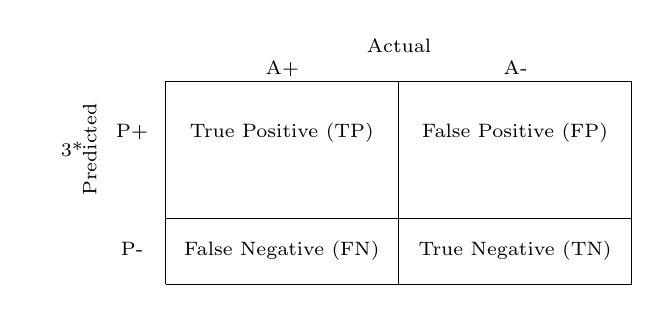
\begin{tikzpicture}[scale=0.4]
      \node at (1,1){
      \scriptsize{
        \begin{tabular}{
            >{\centering}m{1em} >{\centering}m{1em} >{\centering}m{1in} >{\centering\arraybackslash}m{1in}}
          % c>{\centering}m{2em}ccc}
          & & \multicolumn{2}{c}{ Actual}\\
          & & A+ & A- \\
          \cline{3-4}
          & \multicolumn{1}{c|}{} & \multicolumn{1}{c|}{} & \multicolumn{1}{c|}{}\\
          \multirow{3}{*}{\rotatebox[origin=c]{90}{Predicted}}& \multicolumn{1}{c|}{P+} &  \multicolumn{1}{c|}{True Positive (TP)} & \multicolumn{1}{c|}{False Positive (FP)} \\
          &\multicolumn{1}{c|}{}  & \multicolumn{1}{c|}{}& \multicolumn{1}{c|}{} \\
          \cline{3-4}
          & \multicolumn{1}{c|}{} &\multicolumn{1}{c|}{} & \multicolumn{1}{c|}{}\\

          & \multicolumn{1}{c|}{P-} &\multicolumn{1}{c|}{False Negative (FN)}  &\multicolumn{1}{c|}{True Negative (TN)}\\
          & \multicolumn{1}{c|}{} &\multicolumn{1}{c|}{} & \multicolumn{1}{c|}{}\\
          \cline{3-4}
          \end{tabular}
      }};
    \end{tikzpicture}
    \end{center}
\caption{Confusion matrix with true and false positive detected samples (\acs{tp}, \acs{fp}) in the first row, from left to right and the false and true negative detected samples (\acs{fn}, \acs{tn}) in the second row, from left to right.}
\label{fig:CM}
\end{figure}

The details of the experiments are presented from Sect.\,\ref{subsec:exp1} to Sect.\,\ref{subsec:exp4} and summarized in Table~\ref{tab:experiment_summary}.
%In general terms, all the experiments have been carried out using SERI dataset while \emph{Experiment \#1}(Sect.\,\ref{subsec:exp1}) has been complemented using Duke dataset for comparison purposes.
\emph{Experiment \#1}(Sect.\,\ref{subsec:exp1}) is according to the experiment reported in \cite{Lemaintre2015miccaiOCT} to evaluate the effects of different feature representations and compares the results to those obtained by Venhuizen\,\emph{et al.}~\cite{Venhuizen2015}.
\emph{Experiment \#2 and \#3} (Sect.\,\ref{subsec:exp2}\,\&\,\ref{subsec:exp3}) studies the high-level feature representation using \ac{bow}.
The former experiment studies the effect of the codebook size in order to find the optimal number of words using a linear classifier; while the latter compares different classifiers (see Sect.\,\ref{subsec:cls}).
\emph{Experiment \#4} (Sect.\,\ref{subsec:exp4}) solely focus on the low-level representation.

A summary of the most relevant findings can be found in Sect.\,\ref{sec:con}.



\begin{landscape}
  \begin{table}[ht]
\caption{The outline and summary of the performed experiments.}
\medskip
\scriptsize{
\begin{center}
\resizebox{1\linewidth}{!}{
\begin{tabular}{l  c	 c  c  c  c  c  c  c }
\toprule
\\
&  Dataset & Pre-processing & Features & Mapping & Representation & Classification & Validation & Evaluation \\
\cmidrule(l){2-9}
\\
\multirow{3}{*}{Common:} & \multirow{3}{*}{SERI} & \multirow{3}{*}{\ac{nlm}} & \ac{lbp},\ac{lbptop} & \multirow{3}{*}{} & \multirow{3}{*}{}  & & \multirow{3}{*}{\ac{lopocv}}& \multirow{3}{*}{} \\
        &      &          & $S = \{8,16,24\}$ & & & & & \\
        &      &          & $R = \{1,2,3\}$  & & & & & \\\\
\midrule
\\
Experiment\#1:  \\
%\hdashline \noalign{\vskip 3pt}
%\\
\multirow{2}{4cm}{Goal: Evaluation of features, mapping and representation} & \multirow{2}{*}{+ Duke} &\multirow{2}{*}{$\sim$} & \multirow{2}{*}{$\sim$} & \emph{global} & \ac{bow} & \multirow{2}{*}{\ac{rf}} & \multirow{2}{*}{$\sim$} & \multirow{2}{*}{\ac{se}, \ac{sp}, \cite{Venhuizen2015}}\\
&  & & & \emph{local} & Histogram &  & & \\\\
\midrule
\\
Experiment\#2:\\
%\hdashline \noalign{\vskip 3pt}
%\\
\multirow{2}{4cm}{Goal: Finding the optimum number of words}& \multirow{2}{*}{$\sim$} & + \acs{f} & \multirow{2}{*}{$\sim$} & \emph{global} & \multirow{2}{*}{\ac{bow}} & \multirow{2}{*}{\ac{lr}} & \multirow{2}{*}{$\sim$} & \multirow{2}{*}{ \ac{acc}, \ac{f1}}\\
  & & + \acs{fal} & & \emph{local} & & & & \\\\
\midrule
\\
Experiment\#3: \\
%\hdashline \noalign{\vskip 3pt}
%\\
%\hdashline \noalign{\vskip 3pt}
 \multirow{4}{4cm}{Goal: Evaluation of different pre-processing for high-level features }& \multirow{4}{*}{$\sim$} & \multirow{2}{*}{+\acs{f}} & \multirow{4}{*}{$\sim$} & \multirow{2}{*}{\emph{global}} & \multirow{4}{*}{\ac{bow}} & $3$-\ac{nn} & \multirow{4}{*}{$\sim$} & \multirow{4}{*}{\ac{se}, \ac{sp}}\\
 & & \multirow{2}{*}{+\acs{fal}} & & \multirow{2}{*}{\emph{local}} &  & \ac{rf} & & \\
 & & & & & & \ac{svm} & & \\
 & & & & & & \ac{gb} & & \\
\midrule
\\
Experiment\#4:\\
%\hdashline \noalign{\vskip 3pt}
%\\
%\hdashline \noalign{\vskip 3pt}
\multirow{4}{4cm}{Goal: Evaluation of different pre-processing for low-level features} & \multirow{4}{*}{$\sim$} & \multirow{2}{*}{ +\acs{f}} & \multirow{4}{*}{$\sim$} & \multirow{4}{*}{\emph{global}} & \multirow{4}{*}{Histogram} & $3$-\ac{nn} & \multirow{4}{*}{$\sim$} & \multirow{4}{*}{\ac{se}, \ac{sp}}\\
& & \multirow{2}{*}{+\ac{fal}} & & & & \ac{rf} &  &\\
& & & & & & \ac{svm} & & \\
& & & & & & \ac{gb} & & \\
\\
\bottomrule


\end{tabular}}
\end{center}}
\label{tab:table4}
\end{table}
\end{landscape}


\subsection{SERI-Dataset}\label{sec:exp:dataset:seri}
This data was acquired by the Singapore Eye Research Institute (SERI), using CIRRUS TM (Carl Zeiss Meditec, Inc., Dublin, CA) \ac{sdoct} device. The datasets consist of 32 \ac{oct} volumes (16 \ac{dme} and 16 normal cases). Each volume contains 128 B-scan with resolution of 512 $\times$ 1024 pixels.
All \ac{sdoct} images are read and assessed by trained graders and identified as normal or \ac{dme} cases based on evaluation of retinal thickening, hard exudates, intraretinal cystoid space formation and subretinal fluid.

\subsection{Duke-Dataset} \label{sec:exp:dataset:duke}
This dataset, published by Srinivasan\,\emph{et al.}~\cite{Srinivasan2014}, was acquired in Institutional Review Board-approved protocols using Spectralis \ac{sdoct} (Heidelberg Engineering Inc., Heidelberg, Germany) imaging at Duke University, Harvard University and the University of Michigan.
This datasets consist of 45 \ac{oct} volumes (15 \ac{amd}, 15 \ac{dme} and 15 normal). In this study we only consider a subset of the original data containing the 15 \ac{dme} and the 15 normal \ac{oct} volumes.


\subsection{Experiment \#1}\label{subsec:exp1}

% Experiment structure
%
% Intro:
%   - background
%   - goal / experiment intention / why
%   - data
%   - evaluation
%   - reference to result table
%
% Procedure (by data if more than one):
%   - pre-processing
%   - feature extraction
%   - mapping
%   - feature representation
%   - classifier
%
% Result highlights:
%   - (only a description)

%% Experiment intro
This experiment replicates some of the experiments reported in~\cite{Lemaintre2015miccaiOCT}, using the SERI and Duke datasets.
%% Experiment Procedure
The volumes are pre-processed using \nlm.
\lbp and \lbptop descriptors are detected using the default configuration in conjunction with local and global mapping.
Volumes are described using both low-level and high-level feature representation.
In accordance with~\cite{Lemaintre2015miccaiOCT}, \ac{bow} is used with a codebook of size $32$ words, and the volumes are classified using \ac{rf} classifier with 100 un-pruned trees.

Results are listed in Table~\ref{tab:table1-1}.
The two configurations achieving the best results in Table~\ref{tab:table1-1} are compared to Venhuizen\,\textit{et al.}~\cite{Venhuizen2015} in Table~\ref{tab:table1-2}. 
%% Experiment Result description
Overall, the obtained results indicate that features driven from \ac{lbp} descriptors are highly discriminative.
Nevertheless, Table~\ref{tab:table1-2} indicates a substantial performance difference between SERI and Duke dataset.
This is attributed to the fact that the volumes in Duke dataset are provided with embedded pre-processing steps.




  \begin{table}[h]
\caption{ Experiment \#1 - Obtained results of classification using SERI and Duke datasets.}% using \ac{rf} with 100 trees. High-level features with \ac{bow} are obtained with $K$ = 32 visual-words.}
\centering
\resizebox{1\linewidth}{!}{

\begin{tabular}{l lr c lr c lr  c  lr c lr c lr}
\toprule
Features & \multicolumn{8}{c}{SERI dataste} & & \multicolumn{8}{c}{Duke dataset}\\
\cmidrule(l){2-9} \cmidrule(l){11-18}
 	& \multicolumn{2}{c}{$\{8,1\}$}& & \multicolumn{2}{c}{$\{16,2\}$}& &\multicolumn{2}{c}{$\{24,3\}$} & & \multicolumn{2}{c}{$\{8,1\}$}& & \multicolumn{2}{c}{$\{16,2\}$}& &\multicolumn{2}{c}{$\{24,3\}$}\\
  \cmidrule(l){2-3}  \cmidrule(l){5-6}  \cmidrule(l){8-9} \cmidrule(l){11-12}  \cmidrule(l){14-15}  \cmidrule(l){17-18}
	       & \ac{se} & \ac{sp} & & \ac{se} & \ac{sp} & &  \ac{se} & \ac{sp} & &  \ac{se} & \ac{sp} & &  \ac{se} & \ac{sp} & &  \ac{se} & \ac{sp} \\
\midrule
  	%\ac{lbp}					& 43.7 & 43.7 & & 37.5 & 50.0 & & 50.00 & 62.50  \\
 	\emph{global}-\ac{lbptop}				       & 56.2 & 62.5 & & \textbf{87.5} & \textbf{75.0} & & 68.7 & 68.7 & & 80.0 & 93.3 & & 73.3 & 86.6 & & 73.3 & 86.6 \\
	%\ac{lbp}+\ac{bow}		& 50.0 & 81.2 & & 57.5 & 68.7 & & 50.0 & 50.0 \\
	\emph{local}-\ac{lbp}	   & \textbf{75.0} & \textbf{87.5} & & 81.2 & 75.0 & & 68.7 & 62.5 & & \textbf{80.0} & \textbf{86.6} & & \textbf{86.7} & \textbf{100} & & 93.3 & 86.6\\
	\emph{local}-\ac{lbptop}   & 62.5 & 68.7 & & 56.2 & 37.5 & & 37.5 & 43.7 & & 80.0 & 86.6 & & 86.6 & 86.6 & & 60.0 & 80.0 \\
\bottomrule
\end{tabular}}
\label{tab:table1-1}
\end{table}






\begin{table}[h]
\caption{Experment \#1 - Comparing the proposed method by \cite{Venhuizen2015} on SERI and Duke datasets.}% with the \textbf{our two} best proposed methods. $K$ = 32 and \ac{rf} is trained using 100 tress}
\centering
\scriptsize{
\begin{tabular}{l	lr c lr}
\toprule
Data sets 	& \multicolumn{2}{c}{SERI} & & \multicolumn{2}{c}{Duke} \\
  \cmidrule(l){2-3}  \cmidrule(l){5-6}
	         & \ac{se} & \ac{sp} & & \ac{se} & \ac{sp}\\
\midrule
Venhuizen~\textit{et al.} \cite{Venhuizen2015} 		& 61.5 & 58.8 & & 71.4 & 68.7\\
\{\emph{local}-\ac{lbp}\},$8^{riu}$ 				   & \textbf{75.0} & \textbf{87.5} & & \textbf{86.6} & \textbf{100.0}   \\
\{\emph{global}-\ac{lbptop}\},$16^{riu}$				& \textbf{75.0} & \textbf{87.5} & & 80.0 & 86.6  \\


\bottomrule
\end{tabular}}
\label{tab:table1-2}
\end{table}


\subsection{Experiment \#2}\label{subsec:exp2}
% Experiment structure
%
% Intro:
%   - background
%   - goal / experiment intention / why
%   - data
%   - evaluation
%   - reference to result table
%
% Procedure (by data if more than one):
%   - pre-processing
%   - feature extraction
%   - mapping
%   - feature representation
%   - classifier
%
% Remarks (if any)
%
% Result highlights:
%   - (only a description)

%% Experiment intro
In order to determine the optimal size of the codebook when using \bow, this experiment evaluates several codebook sizes on SERI dataset.

%% Experiment procedure
Several pre-processing strategies are evaluated: (i) \nlm, (ii) a combination of \nlm and flattening, and (iii) a combination of \nlm, flattening and aligning.
\lbp and \lbptop descriptors are detected using the default configuration.
Volumes are represented using \ac{bow}, where the codebook size ranging for $k \in \{10, 20, 30, \cdots, 100, 200, \cdots, 500, 1000\}$.
Finally, the volumes are classified using \lr.
The choice of this linear classifier avoids that the results get boosted by the classifier. In this manner any improvement would be linked to the pre-processing and the size of the codebook.

\begin{landscape}
  \begin{table}
\caption{Experiment \#1 - Optimum number of words for each configuration as a result of \ac{lr} Classification, for high-level feature extraction of \emph{global} and \emph{local}-\ac{lbp}, and \emph{local}-\ac{lbptop} features with different pre-processing. The pre-processing includes: \ac{nf}, \ac{f}, and \ac{fal}.
The achieved performances are indicated in terms of  \acs{acc}, \acs{f1}, \acs{se}, and \acs{sp}}
\centering

\footnotesize{
\resizebox{1\linewidth}{!}{
\begin{tabular}{ll  ccccr	c	ccccr	c ccccr}
\toprule
Features & Pre-processing &    \multicolumn{5}{c}{$\{8,1\}$}  & & \multicolumn{5}{c}{$\{16,2\}$} & & \multicolumn{5}{c}{$\{24,3\}$} \\
  \cmidrule(l){3-7}  \cmidrule(l){9-13}  \cmidrule(l){15-19}
   & &  	\ac{acc}\% & \ac{f1}\% & \ac{se}\% & \ac{sp}\%  & W\# &  & \ac{acc}\% & \ac{f1}\% & \ac{se}\% & \ac{sp}\%  & W\# &  &\ac{acc}\% & \ac{f1}\% & \ac{se}\% & \ac{sp}\%  & W\# \\
\midrule
\\[-2ex]
  	\emph{global}-\ac{lbp}		\\
 	& \acs{nf} & 81.2 &  78.5 & 68.7 &  93.7 & 500 & & 62.5 & 58.0 & 56.2 & 62.5 & 80  & & 62.5  & 62.5 & 62.5 & 62.5 & 80  \\
	& \acs{f}  & 71.9 &  71.0 & 68.7 &  75.0 & 400 & & 68.7 & 66.7 & 62.5 & 75.0 & 300 & & 68.7  & 66.7 & 62.5  & 75.0 & 300	 \\
	& \acs{fal}& 71.9 &  71.0 & 68.7 &  75.0 & 500 & & 71.9 & 71.0 & 68.7 & 75.0 & 200 & & 75.0  & 68.7 & 68.7  & 68.7 & 500	 \\
	%& \acs{fac}& 75.0 & 73.3 & 68.7 &  81.2 & 500 & & 78.1 & 75.8 & 68.7 & 87.5 & 500 & & 68.7  & 68.7 & 68.7  & 68.7 & 90	 \\
	\\
\hdashline \noalign{\vskip 3pt}
\\[-2ex]
 	\emph{local}-\ac{lbp}		\\
 	& \acs{nf}  & 75.0  & 75.0 & 75.0  & 75.0 & 70 & & 65.6 & 64.5 & 62.5 & 68.7 & 90 & &  62.5 & 60.0 & 56.2  & 68.7  & 30  \\
	& \acs{f}   & 75.0  & 73.3 & 68.7  & 81.2 & 30 & & 71.8 & 61.0 & 68.7 & 75.0 & 70 & &  62.5 & 62.5 & 62.5  & 62.5  & 100	 \\
	& \acs{fal} & 75.0  & 69.0 & 62.5  & 81.2 & 40 & & 71.9 & 71.0 & 68.7 & 75.0 & 200 & &  68.7 & 66.7 & 68.7 & 62.5 & 10	 \\
	%& \acs{fac}& 68.7 & 68.7 & 68.7 & 68.7 & 300 & & 65.6 & 64.5 & 62.5 & 68.7 & 100 & & 65.6  & 64.5 & 62.5  & 68.7 & 100	 \\
	\\
\hdashline \noalign{\vskip 3pt}
\\[-2ex]
 	\emph{local}-\ac{lbptop}		\\
 	& \acs{nf}	& 68.7 & 68.7 & 68.7 & 68.7 & 400 & & 75.0  & 75.0   & 75.0   & 75.0  & 500 & & 71.9 & 71.0 & 68.7 & 75.0 & 60	 \\
	& \acs{f}	& 68.7 & 68.7 & 68.7 & 68.7 & 300 & & 68.7  & 66.7   & 62.5   & 75.0  & 50  & & 75.0 & 76.5 & 81.2 & 68.7 & 80	 \\
	& \acs{fal}	& 75.0 & 73.3 & 68.7 & 81.2 & 100 & & 75.0  & 73.3   & 68.7   & 81.2  & 90  & & 75.0 & 69.0 & 62.5 & 81.2 & 70	 \\
	%& \acs{fac}	& 71.9 & 69.0 & 62.5 & 81.2 & 400 & & 75.0  & 73.3   & 68.7   & 81.2  & 100 & & 75.0 & 73.3 & 68.7 & 81.2 & 60	 \\
	\\

\bottomrule
\end{tabular}}}
\label{tab:table2}
\end{table}
\end{landscape}


%\begin{tiny}
  \begin{table}[ht]
\caption{Experiment \#2 - The obtained results, using the optimal number of words in terms of \ac{se} and \ac{sp}.}
\centering

\footnotesize{
\resizebox{1\linewidth}{!}{
\begin{tabular}{ll  lcr	c	lcr	c lcr}
\toprule
Features & Pre-processing &    \multicolumn{3}{c}{$\{8,1\}$}  & & \multicolumn{3}{c}{$\{16,2\}$} & & \multicolumn{3}{c}{$\{24,3\}$} \\
  \cmidrule(l){3-5}  \cmidrule(l){7-9}  \cmidrule(l){11-13}
   & &  	\ac{se}\% & \ac{sp}\% & W\# &  & \ac{se}\% & \ac{sp}\% & W\# &  & \ac{se}\% & \ac{sp}\% & W\#\\
\midrule
  	\emph{global}-\ac{lbp}		\\
 	& \acs{nf} & 68.7 &  93.7 &  500 & & 56.2 & 62.5 & 80  & & 62.5  & 62.5 & 80  \\
	& \acs{f}  & 68.7 &  75.0 &  400 & & 62.5 & 75.0 & 300 & & 62.5  & 75.0 & 300	 \\
	& \acs{fal}& 68.7 &  75.0 &  500 & & 68.7 & 75.0 & 200 & & 68.7  & 68.7 & 500	 \\
	%& \acs{fac}& 68.7   &  81.2 &  500 & & 68.7 & 87.5  & 500 & & 68.7  & 68.7 & 90	 \\
\hdashline \noalign{\vskip 3pt}
 	\emph{local}-\ac{lbp}		\\
 	& \acs{nf} & 75.0  & 75.0 & 70 & & 62.5 & 68.7  & 90 & &  56.2  & 68.7   & 30  \\
	& \acs{f}  & 68.7  & 81.2 & 30 & & 68.7 & 75.0  & 70 & &  62.5  & 62.5 & 100	 \\
	& \acs{fal} & 62.5 & 81.2 & 40 & & 68.7 & 75.0  & 200 & &  68.7 & 62.5 & 10	 \\
	%& \acs{fac}& 68.7 & 68.7 & 300 & & 62.5 & 68.7 & 100 & & 62.5  & 68.7 & 100	 \\
\hdashline \noalign{\vskip 3pt}
 	\emph{local}-\ac{lbptop}		\\
 	& \acs{nf}	& 68.7 & 68.7 & 400 & & 75.0   & 75.0   & 500 & & 68.7 & 75.0 &60	 \\
	& \acs{f}	& 68.7 & 68.7 & 300 & & 62.5   & 75.0 & 50  & & 81.2   & 68.7  & 80	 \\
	& \acs{fal}	& 68.7 & 81.2 & 100 & & 68.7   & 81.2 & 90  & & 62.5   & 81.2 &  70	 \\
	%& \acs{fac}	& 62.5 & 81.2   & 400 & & 68.7   & 81.2 & 100 & & 68.7   & 81.2 &60	 \\

\bottomrule
\end{tabular}}}
\label{tab:table2-2}
\end{table}
%\end{tiny}



The usual build of the codebook consists of clustering the samples in
the feature space using $k$-means (see Sect.\,\ref{subsec:fearep}).
However, this operation is rather computationally expensive and convergence of the $k$-means algorithm for all codebook sizes is not granted.
Nonetheless, Nowak\,\textit{et al.}~\cite{nowak2006sampling} pointed out that randomly generated codebooks can be used at the expenses of accuracy.
Thus, the codebook are randomly generated since the final aim is to asses the influence of codebook size and not the performance of the framework.
For this experiment, the codebook building is carried out using random initialization $k$-means++ algorithm~\cite{arthur2007k}, which is usually used as a $k$-means initialization algorithm.

Figure~\ref{fig:RBOW} shows the \ac{acc} and \ac{f1} score graphs obtained for a single case \footnote{Full set of scores can be found at the github repository} in~\cite{Lemaitre2015}, while the optimal number of words for all the configuration are reported in a compact manner in Table~\ref{tab:table2}.
Table~\ref{tab:table2-2} reports the performance of the optimal codebook size in terms of \ac{se} and \ac{sp}.

\begin{figure}
\centering
\includegraphics[width=0.85\textwidth]{figure2}
\caption{The performance of \ac{lr} with \ac{nlm}+\ac{f} pre-processing for different $P$ and $R$.}
\label{fig:RBOW}
\end{figure}


%% Experiment Result description
The obtained results show that commonly less number of words is required when higher number of sampling points and radius ($\{P,R\} = \{24,3\}$) are used.
The required number of words decreases for \emph{local}-\ac{lbp} in comparison with \emph{global}-\ac{lbp}.
Although it was expected that the use of different pre-processing steps affect the optimal number of words, this influence is not substantial nor consistent over all the obtained results.


\subsection{Experiment \#3}\label{subsec:exp3}
% Experiment structure
%
% Intro:
%   - background
%   - goal / experiment intention / why
%   - data
%   - evaluation
%   - reference to result table
%
% Procedure (by data if more than one):
%   - pre-processing
%   - feature extraction
%   - mapping
%   - feature representation
%   - classifier
%
% Remarks (if any)
%
% Result highlights:
%   - (only a description)

%% Experiment intro
After studying the impact of the codebook size in Sect.\,\ref{subsec:exp2}, this experiment explores the improvement associated with: (i) different pre-processing, and (ii) using larger range of classifiers (i.e. linear and non-linear).

%% Procedure
For this experiment, several pre-processing strategies are evaluated: (i) \nlm, (ii) a combination of \nlm and flattening, and (iii) a combination of \nlm, flattening and aligning.
\lbp and \lbptop features are detected using the default configuration and volumes are represented using \bow.
The codebooks are computed using regular $k$-means algorithm which is initialized using $k$-means++, where $k$ is chosen according to the findings of \emph{Experiment \#2}.
Finally, the volumes are classified using $k$-\ac{nn}, \ac{rf}, \ac{gb}, and \ac{svm}.

Regarding the classification strategies, $k$-\ac{nn} classifier is trained by considering the 3 nearest neighbor.
The \ac{rf} and \ac{gb} classifier are trained using 100 un-pruned trees, while \ac{svm} classifier is trained with \ac{rbf} kernel and its parameters $C$, and $\gamma$ are optimized through grid-search.

%% Experiment Result description
Table~\ref{tab:table3} shows the obtained results from this experiment, where the most relevant configurations are shaded and the highest results are highlighted in \textbf{bold}.
Regarding the effects of pre-processing, the performance of the most configurations decreases by aligning or flattening the B-scan (i.e. light shaded configurations in Table~\ref{tab:table3}).
%$k$-NM\,8\,\emph{local}-\lbp, \svm\,8\,\emph{local}-\lbptop, \svm\,16\,\emph{local}-\lbptop, \rf\,8\,\emph{global}-\lbp, \rf\,8\,\emph{local}-\lbp).
However, the two best configurations (i.e. dark shaded in Table~\ref{tab:table3}), achieve better results when adding flattening or flattening and alignment as pre-processing.
A small radius and small number of samples in feature detection tends to increase the classification performance.
%(see: \svm\,8\,\emph{local}-\lbp and \rf\,16\,\emph{local}-\lbptop).
%Feature detection shows a tendency towards better results when using small radius and small number of samples.
Regarding the mapping strategy, local mapping tends to produce better results than global mapping.
In terms of choosing a classifier, \ac{svm} provides the best results, followed by \rf.

The best results (81.2\%\,\ac{se} and 93.7\%\,\ac{sp}) are achieved using \nlm, flattening, \lbp detection using $\{P,R\} = \{8,1\}$, local mapping, high-level representation, using a codebook with $k=70$, and \svm classifier.
This result can be compared with other relevant results in Table\,\ref{tab:experiment_summary}.

\subsection{Experiment \#4}\label{subsec:exp4}
% Experiment structure
%
% Intro:
%   - background
%   - goal / experiment intention / why
%   - data
%   - evaluation
%   - reference to result table
%
% Procedure (by data if more than one):
%   - pre-processing
%   - feature extraction
%   - mapping
%   - feature representation
%   - classifier
%
% Remarks (if any)
%
% Result highlights:
%   - (only a description)

%% Experiment intro
This experiment replicates the \emph{Experiment \#3} for the case of low-level representation features from the volumes.

%% Experiment procedure
For this experiment, several pre-processing strategies are evaluated: (i) \nlm, (ii) a combination of \nlm and flattening, and (iii) a combination of \nlm, flattening and aligning.
\lbp and \lbptop descriptors are detected using the default configuration.
Volumes are represented using low-level feature representation of the \emph{global} mapping.
Finally, the volumes are classified using $k$-\ac{nn}, \ac{rf}, \ac{gb}, and \ac{svm}, similarly to \emph{Experiment \#3}.

%% Experiment Result description
The obtained results from this experiment is listed in Table.~\ref{tab:table4}.
The most relevant configurations are shaded and the highest results are highlighted in \textbf{bold}.
Similarly to the results reported in Sect.\,\ref{subsec:exp3}, the effect of flattening the B-scan boosts the results for the best performing configuration, but this effect is not consistent across all the configurations.
For this experiment, \lbptop outperforms \lbp and larger $P$ and $R$ values for feature detection tends to obtain better results. 
In terms of classifier, \rf have better performance than the others but the highest \ac{sp} is achieved using \svm.


% The highest results of this experiment, \ac{se} and \ac{sp} of 81.2\% and 81.2\%, respectively, was achieved with \ac{rf} and using \emph{global}-\ac{lbptop} features with sampling points and radius of $\{S,R\}=\{24,3\}$.
% In general, in this experiment, \emph{global}-\ac{lbptop} features have better performance in comparison to \emph{global}-\ac{lbp} features and the  classification rates improved while using a higher number of sampling points and radius ($\{S,R\}=\{24,3\}$).

% Similar to the previous experiments, although the effects of additional pre-processing steps (\ac{f} and \ac{fal}) is evident for \ac{rf} performance on $\{S,R\} = \{24,3\}$, similar to the previous experiments, this influence is not consistent for all different configurations, in terms of classifier and $\{S,R\}$.


The best results (81.2\%\,\ac{se} and 81.2\%\,\ac{sp}) are achieved when using \nlm, flattening, \lbptop detection using $\{P,R\}= \{24,3\}$, global mapping, low-level representation, and \rf classifier.
This result can be compared with other relevant results in Table\,\ref{tab:experiment_summary}

\begin{landscape}
  \begin{table}[ht]
\caption{Experiment \#3 - $k$-\ac{nn} and  \ac{svm} classification with \ac{bow} for the \emph{global} and \emph{local} \ac{lbp} and \emph{local} \ac{lbptop} features with different pre-processing. The optimum number of words were selected based on the previous experiment.}
\centering

\scriptsize{
\resizebox{0.9\linewidth}{!}{
\begin{tabular}{ll  lr	c	lr	c lr c lr	c	lr	c lr}
\toprule
& & \multicolumn{8}{c}{$k$-\ac{nn}} & & \multicolumn{8}{c}{\ac{svm}}\\
\cmidrule(l){3-10} \cmidrule(l){12-19}
Features & Pre-processing &    \multicolumn{2}{c}{$\{8,1\}$}  & & \multicolumn{2}{c}{$\{16,2\}$} & & \multicolumn{2}{c}{$\{24,3\}$}  & &   \multicolumn{2}{c}{$\{8,1\}$}  & & \multicolumn{2}{c}{$\{16,2\}$} & & \multicolumn{2}{c}{$\{24,3\}$} \\
  \cmidrule(l){3-4}  \cmidrule(l){6-7}  \cmidrule(l){9-10}   \cmidrule(l){12-13}  \cmidrule(l){15-16}  \cmidrule(l){18-19}
   & &  	\ac{se}\% & \ac{sp}\% &  & \ac{se}\% & \ac{sp}\% &  & \ac{se}\% & \ac{sp}\%  & & 	\ac{se}\% & \ac{sp}\% &  & \ac{se}\% & \ac{sp}\% &  & \ac{se}\% & \ac{sp}\% \\
\midrule
  	\emph{global}-\ac{lbp}		\\
 	& \acs{nf} & 43.7 &  93.7 &   & 43.7 & 87.5  &  & 43.7  & 62.5  &  & 68.7 & 87.5 & & 62.5 & 62.5 & & 50.0 & 56.2 \\  
	& \acs{f}  & 43.7 &  56.2 &   & 50.0 & 75.0  &  & 62.5  & 56.2  &  & 56.2 & 56.2 & & 56.2 & 75.0 & & 56.2 & 68.7  \\
	& \acs{fa} & 56.2 &  62.5 &   & 43.7 & 81.2  &  & 68.7  & 56.2  &  & 56.2 & 68.7 & & 68.7 & 68.7 & & 56.2 & 75.0	 \\
	%& \acs{fac}& 50   &  75.0 &   & 37.5 & 87.5  &  & 50.0  & 62.5 &  & 50.0 & 75.0 & & 50.0 & 75.0 & & 43.7 & 68.7 \\
\hdashline \noalign{\vskip 3pt}
 	\emph{local}-\ac{lbp}		\\
 	& \acs{nf} & \cellcolor[gray]{0.8}\textbf{75.0} & \cellcolor[gray]{0.8}\textbf{87.5} & & 50.0  & 68.7 &  &  43.7  & 43.7 & & \cellcolor[gray]{0.6}\textbf{75.0} & \cellcolor[gray]{0.6}\textbf{93.7} & & 50.0 & 75.0 & & 56.2 & 56.2    \\
	& \acs{f}  & \cellcolor[gray]{0.8}56.2 & \cellcolor[gray]{0.8}56.2 & & 50.0  & 50.0 &  & 50.0   & 43.7 & &\cellcolor[gray]{0.6}\textbf{81.2} & \cellcolor[gray]{0.6}\textbf{93.7} & & 68.7 & 68.7 & & 68.7 & 75.0 \\
	& \acs{fa} & \cellcolor[gray]{0.8}56.2 & \cellcolor[gray]{0.8}43.7 & & 50.0  & 75.0 &  & 50.0   & 62.5 & & \cellcolor[gray]{0.6}\textbf{75.0} & \cellcolor[gray]{0.6}\textbf{93.7} & & 75.0 & 68.7 & & 68.7 & 68.7  \\
	%& \acs{fac}& 37.5 & 75.0 & & 31.2 & 75.0 &  & 62.5  & 81.2 & & 62.5 & 87.5 & & 56.2 & 43.7 & & 75.0 & 56.2	 \\
\hdashline \noalign{\vskip 3pt}
 	\emph{local}-\ac{lbptop}		\\
 	& \acs{nf} & 56.2 & 75.0 & & 56.2 & 75.0 & & 62.5 & 56.2 & & \cellcolor[gray]{0.8}\textbf{81.2} & \cellcolor[gray]{0.8}\textbf{87.5} & & \cellcolor[gray]{0.8}\textbf{75.0} & \cellcolor[gray]{0.8}\textbf{100} & & 56.2 & 75.0 \\
	& \acs{f} & 62.5 & 43.7 & & 37.5 & 68.7 & & 43.7 & 62.5 & & \cellcolor[gray]{0.8}\textbf{81.2} & \cellcolor[gray]{0.8}\textbf{81.2} & & \cellcolor[gray]{0.8}75.0 & \cellcolor[gray]{0.8}68.7 & & 81.2 & 68.7		 \\
	& \acs{fal}	& 56.2 & 56.2 & & 68.7 & 50.0 & & 43.7 & 62.5 & & \cellcolor[gray]{0.8}62.5 & \cellcolor[gray]{0.8}75.0 & & \cellcolor[gray]{0.8}68.7 & \cellcolor[gray]{0.8}75.0 & & 62.5 & 81.2  \\
	%& \acs{fac} & 43.7 & 68.7 & & 68.7 & 75.0 & & 56.2 & 81.2 & & 56.2 & 87.5 & & 87.5 & 75.0 & & 62.5 & 75.0	 	 \\
\midrule
& & \multicolumn{8}{c}{\ac{rf}} & & \multicolumn{8}{c}{\ac{gb}}\\
\cmidrule(l){3-10} \cmidrule(l){12-19}
Features & Pre-processing &    \multicolumn{2}{c}{$8^{riu2}$}  & & \multicolumn{2}{c}{$16^{riu2}$} & & \multicolumn{2}{c}{$24^{riu2}$}  & &   \multicolumn{2}{c}{$8^{riu2}$}  & & \multicolumn{2}{c}{$16^{riu2}$} & & \multicolumn{2}{c}{$24^{riu2}$} \\
  \cmidrule(l){3-4}  \cmidrule(l){6-7}  \cmidrule(l){9-10}   \cmidrule(l){12-13}  \cmidrule(l){15-16}  \cmidrule(l){18-19}
   & &  	\ac{se}\% & \ac{sp}\% &  & \ac{se}\% & \ac{sp}\% &  & \ac{se}\% & \ac{sp}\%  & & 	\ac{se}\% & \ac{sp}\% &  & \ac{se}\% & \ac{sp}\% &  & \ac{se}\% & \ac{sp}\% \\
\midrule
  	\emph{global}-\ac{lbp}		\\
 	& \acs{nf} & \cellcolor[gray]{0.8}\textbf{68.7} & \cellcolor[gray]{0.8}\textbf{93.7} & & 43.7 & 62.5 & & 50.0 & 68.7  & & 56.2 & 50.0 & & 37.5 & 31.2 & & 50.0 & 43.7\\
	& \acs{f}  & \cellcolor[gray]{0.8}56.2 & \cellcolor[gray]{0.8}50.0 & & 56.2 & 75.0 & & 50.0 & 75.0  & & 50.0 & 56.2 & & 56.2 & 75.0 & & 43.7 & 62.5\\
	& \acs{fa} & \cellcolor[gray]{0.8}68.7 & \cellcolor[gray]{0.8}50.0 & & 56.2 & 62.5 & & 62.5 & 56.2  & & 56.2 & 50.0 & & 68.7 & 50.0 & & 43.7 & 75.0\\
	%& \acs{fac} & 68.7 & 68.7 & & 56.2 & 75.0 & & 50.0 & 68.7& &  50.0 & 68.7 & & 75.0 & 62.5 & & 56.2 & 81.2  \\ 
\hdashline \noalign{\vskip 3pt}
 	\emph{local}-\ac{lbp}		\\
 	& \acs{nf} &  \cellcolor[gray]{0.8}\textbf{81.2} & \cellcolor[gray]{0.8}\textbf{81.2} & & 62.5 & 56.2 & & 56.2 & 56.2 & & 75.0 & 62.5 & & 68.7 & 87.5 & & 50.0 & 75.0   \\
	& \acs{f}  &  \cellcolor[gray]{0.8}56.2 & \cellcolor[gray]{0.8}81.2 & & 62.5 & 68.7 & & 68.7 & 62.5 & & 68.7 & 75.0 & & 50.0 & 75.0 & & 50.0 & 62.5 \\
	& \acs{fa} &  \cellcolor[gray]{0.8}68.7 & \cellcolor[gray]{0.8}62.5 & & 62.6 & 68.7 & & 43.7 & 43.7 & & 56.2 & 50.0 & & 68.7 & 56.2 & & 50.0 & 50.0 \\
	%& \acs{fac}&  62.5 & 68.7 & & 68.7 & 68.7 & & 68.7 & 56.2 & &  56.2 & 50.0 & & 56.2 & 68.7 & & 62.5 & 68.7  \\
\hdashline \noalign{\vskip 3pt}
 	\emph{local}-\ac{lbptop}		\\
 	& \acs{nf} & 68.7 & 62.5 & & \cellcolor[gray]{0.6}\textbf{68.7} & \cellcolor[gray]{0.6}\textbf{81.2} & & 68.7 & 68.7 & & 37.5 & 68.7 & & 62.5 & 81.2 & & 62.5 & 50.0  \\
	& \acs{f} & 50.0 & 62.5 & & \cellcolor[gray]{0.6}62.5 & \cellcolor[gray]{0.6}62.5 & & 43.7 & 75.0 & & 50.0 & 56.2 & & 43.7 & 62.5 & & 50.0 & 62.5		 \\
	& \acs{fal}	& 50.0 & 62.5 & & \cellcolor[gray]{0.6}\textbf{81.2} & \cellcolor[gray]{0.6}\textbf{87.5} & & 50.0 & 68.7 & & 56.2 & 62.5 & & 81.2 & 68.7 & & 75.0 & 68.7  \\
	%& \acs{fac}	 & 56.2 & 81.2 & & 68.2 & 81.2 & & 68.7 & 87.5 & & 75.0 & 68.7 & & 87.5 & 75.0 & & 75.0 & 87.5 	 \\

\bottomrule
\end{tabular}}}
\label{tab:table3}
\end{table}
%\end{tiny}
\end{landscape}

%--------------------------------------------------------
%  \begin{table}[ht]
%\caption{The obtained results of experiment \#2.
%Classification results obtained from low-level representation of global \ac{lbp} and \ac{lbptop} features with different pre-processing.
%Pre-processing steps include: \ac{nf}, \ac{f}, \ac{fal}, and \ac{fac}.
%Different classifiers such as \ac{rf}, \ac{gb}, \ac{svm}, \ac{lr}, and $k$-\ac{nn} are used.
%}
%\medskip
%
%\footnotesize{
%\begin{center}
%\resizebox{1\linewidth}{!}{
%%\begin{tabularx}{1.02\linewidth}{l cc  cc cc c cc cc cc }
%\begin{tabular}{l cc  cc cc c cc cc cc }
%\toprule
%& \multicolumn{6}{c}{\ac{rf}} & &  \multicolumn{6}{c}{\ac{gb}} \\
%\cmidrule(l){2-7} \cmidrule(l){9-14}
%Features &  \multicolumn{2}{c}{$8^{riu2}$}  & \multicolumn{2}{c}{$16^{riu2}$} & \multicolumn{2}{c}{$24^{riu2}$} & &  
%   \multicolumn{2}{c}{$8^{riu2}$}  &  \multicolumn{2}{c}{$16^{riu2}$} & \multicolumn{2}{c}{$24^{riu2}$} \\
%  \cmidrule(l){2-3}  \cmidrule(l){4-5}  \cmidrule(l){6-7} \cmidrule(l){9-10}  \cmidrule(l){11-12}  \cmidrule(l){13-14}
%   &  	\ac{se}\% &  \ac{sp}\%  &  \ac{se}\% &  \ac{sp}\% & 	\ac{se}\% &  \ac{sp}\% & & 
%   \ac{se}\% &  \ac{sp}\% & \ac{se}\% &  \ac{sp}\% & \ac{se}\% &  \ac{sp}\%\\
%\midrule
%  	\emph{global}-\ac{lbp} \\
% 	\acs{nf} & 43.7 & 62.5 &   43.7 & 62.5 & 56.2 & 75   & &  43.7 & 43.7 & 43.7 & 37.5 & 37.5 & 31.25  		\\
%	\acs{f}  & 56.2 & 56.2 &   68.7 & 62.5 & 62.5 & 68.7 & &  25   & 56.2 & 50   & 43.7 & 25   & 43.7 \\
%	\acs{fa} & 65.2 & 56.2 &   50   & 50   & 56.2 & 68.7 & &  43.75& 62.5 & 62.5 & 50   & 31.2 & 31.2 \\
%	\acs{fac}& 56.2 & 62.5 &   56.2 & 62.5 & 68.7 & 56.2 & &  25   & 62.5 & 75   & 81.2 & 93.7 & 87.5\\
%
%\hdashline \noalign{\vskip 3pt}
% 	\emph{global}-\ac{lbptop}		\\
% 	\acs{nf}	 & 56.2 & 68.7 &   68.7  & 87.5 & 68.7  & 81.2 & &  68.7 & 68.7 & 75   & 50   & 56.2 & 43.7\\
%	\acs{f}	 & 56.2 & 62.5 &   81.2  & 68.7 & 81.2  & 81.2 & &  56.2 & 62.5 & 62.5 & 68.7 & 68.7 & 81.2\\
%	\acs{fal}& 68.7 & 62.5 &   75    & 68.7 & 75    & 81.2 & &  56.2 & 43.7 & 62.5 & 62.5 & 75   & 75 \\
%	\acs{fac}& 75   & 68.7 &   75    & 81.2 & 75    & 75   & &  75   & 75   & 75   & 56.2 & 81.2 & 62.5\\
%\midrule
%& \multicolumn{6}{c}{\ac{svm}} & &  \multicolumn{6}{c}{$k$-\ac{nn}} \\
%\cmidrule(l){2-7} \cmidrule(l){9-14}
%Features &  \multicolumn{2}{c}{$8^{riu2}$}  & \multicolumn{2}{c}{$16^{riu2}$} & \multicolumn{2}{c}{$24^{riu2}$} & &  
%   \multicolumn{2}{c}{$8^{riu2}$}  &  \multicolumn{2}{c}{$16^{riu2}$} & \multicolumn{2}{c}{$24^{riu2}$} \\
%  \cmidrule(l){2-3}  \cmidrule(l){4-5}  \cmidrule(l){6-7} \cmidrule(l){9-10}  \cmidrule(l){11-12}  \cmidrule(l){13-14}
%   &  	\ac{se}\% &  \ac{sp}\%  &  \ac{se}\% &  \ac{sp}\% & 	\ac{se}\% &  \ac{sp}\% & & 
%   \ac{se}\% &  \ac{sp}\% & \ac{se}\% &  \ac{sp}\% & \ac{se}\% &  \ac{sp}\%\\
%\midrule
%  	\emph{global}-\ac{lbp}		\\
% 	\acs{nf} & 56.2 & 62.5 & 56.2 & 43.7 & 56.2 & 68.7 & & 37.5 & 50   & 25   & 50   & 37.5 & 68.7 \\
%	\acs{f}  & 75   & 68.7 & 62.5 & 62.5 & 62.5 & 68.7 & & 62.5 & 50   & 56.2 & 75   & 62.5 & 68.7\\
%	\acs{fa} & 75   & 68.7 & 62.5 & 62.5 & 62.5 & 68.7 & & 56.2 & 50   & 56.2 & 75   & 62.5 & 68.7 \\
%	\acs{fac}& 56.2 & 62.5 & 25   & 50   & 43.7 & 62.5 & & 50   & 43.7 & 68.7 & 62.5 & 62.5 & 62.5\\
%
%\hdashline \noalign{\vskip 3pt}
% 	\emph{global}-\ac{lbptop}		\\
% 	\acs{nf}	  & 62.5 & 75   & 62.5 & 93.7 & 56.2 & 87.5 & & 31.2 & 93.7 & 37.5 & 100  & 37.5 & 81.2 \\
%	\acs{f}	  & 68.7 & 75   & 43.7 & 68.7 & 68.7 & 56.2 & & 50   & 56.2 & 56.2 & 75   & 56.2 & 62.5\\
%	\acs{fal} & 68.7 & 62.5 & 62.5 & 56.2 & 56.2 & 68.7 & & 75   & 43.7 & 56.2 & 43.7 & 68.7 & 50  \\
%	\acs{fac} & 68.7 & 68.7 & 68.7 & 87.5 & 68.7 & 87.5 & & 62.5 & 62.5 & 68.7 & 68.7 & 75   & 75\\
%%\midrule
%%
%%& \multicolumn{6}{c}{\ac{lr}} \\
%%\cmidrule(l){2-7} 
%%Features &  \multicolumn{2}{c}{$8^{riu2}$}  & \multicolumn{2}{c}{$16^{riu2}$} & \multicolumn{2}{c}{$24^{riu2}$}  \\
%%  \cmidrule(l){2-3}  \cmidrule(l){4-5}  \cmidrule(l){6-7} 
%%   &  	\ac{se}\% &  \ac{sp}\%  &  \ac{se}\% &  \ac{sp}\% & 	\ac{se}\% &  \ac{sp}\% \\
%%\midrule
%%
%%\emph{global}-\ac{lbp}		\\
%%	\acs{nf}	  & 56.2 & 43.7 & 43.7 & 56.2 & 50 & 68.7\\
%%	\acs{f}	  & 56.2 & 43.7 & 56.2 & 37.5 & 68.7 & 43.7 \\
%%	\acs{fal} & 56.2 & 43.7 & 56.2 & 31.2 & 68.7 & 43.7 \\
%%	\acs{fac} & 62.5 & 56.2 & 56.2 & 62.5 & 56.2 & 56.2\\
%%
%%
%%\hdashline \noalign{\vskip 3pt}
%% 	\emph{global}-\ac{lbptop}		\\
%% 	\acs{nf}  & 50   & 50 &  6 & 93.7 & 0 & 100	\\
%%	\acs{f}	  & 75   & 18 & 50 & 75 & 25 & 81.2\\
%%	\acs{fal} & 93.7 & 6  & 93.7 & 6 & 50 & 43.7\\
%%	\acs{fac} & 50   & 81.2 & 0 & 93.7 & 0 & 100\\
%
%\bottomrule
%
%
%\end{tabular}}
%
%\end{center}}
%\label{tab:table4}
%\end{table}
%\begin{tiny}
  \begin{table}[ht]
\caption{The obtained results of experiment \#4.
Classification results obtained from low-level representation of global \ac{lbp} and \ac{lbptop} features with different pre-processing.
Pre-processing steps include: \ac{nf}, \ac{f}, \ac{fal}, and \ac{fac}.
Different classifiers such as \ac{rf}, \ac{gb}, \ac{svm}, \ac{lr}, and $k$-\ac{nn} are used.
}
\medskip
\scriptsize{
\begin{center}
\begin{tabularx}{1.02\linewidth}{l c  lcr cc lcr cc lcr ccc lcr cc lcr cc lcr }
\toprule
& \multicolumn{13}{c}{\ac{rf}} & & & & \multicolumn{13}{c}{\ac{gb}} \\
\cmidrule(l){2-15} \cmidrule(l){18-31}
Features &  &    \multicolumn{3}{c}{$8^{riu2}$}  & & & \multicolumn{3}{c}{$16^{riu2}$} & & & \multicolumn{3}{c}{$24^{riu2}$} & & & & 
   \multicolumn{3}{c}{$8^{riu2}$}  & & & \multicolumn{3}{c}{$16^{riu2}$} & & & \multicolumn{3}{c}{$24^{riu2}$} \\
  \cmidrule(l){2-5}  \cmidrule(l){7-10}  \cmidrule(l){12-15} \cmidrule(l){18-21}  \cmidrule(l){23-26}  \cmidrule(l){28-31}
   &  & 	\ac{se}\% &  & \ac{sp}\%  &  &  & 	\ac{se}\% &  & \ac{sp}\% & & & 	\ac{se}\% &  & \ac{sp}\% & & & & 
   \ac{se}\% &  & \ac{sp}\% & & & 	\ac{se}\% &  & \ac{sp}\% & & &  	\ac{se}\% &  & \ac{sp}\%\\
\midrule
  	\emph{global}-\ac{lbp} \\
 	\acs{nf} &  & 43.7 & & 62.5 & & & 43.7 &  & 62.5 & & & 56.2 & & 75 & & & & 43.7 & & 43.7 & & & 43.7 & & 37.5 & & & 37.5 & & 31.25  		\\
	\acs{f}  &  & 56.2 & & 56.2 & & & 68.7 & & 62.5 & & & 62.5 & & 68.7 & & & & 25 & & 56.2 & & & 50 & & 43.7 & & & 25 & & 43.7 \\
	\acs{fa} &  & 65.2 & & 56.2 & & & 50 & & 50 & & & 56.2 & & 68.7 & & & & 43.75 & & 62.5 & & & 62.5 & & 50 & & & 31.2 & & 31.2 \\
	\acs{fac}&  & 56.2 & & 62.5 & & & 56.2 & & 62.5 & & & 68.7 & & 56.2 & & & & 25 & & 62.5 & & & 75 & & 81.2 & & & 93.7 & & 87.5\\

\hdashline \noalign{\vskip 3pt}
 	\emph{global}-\ac{lbptop}		\\
 	\acs{nf}	 & & 56.2 & & 68.7 & & & 68.7 & & 87.5 & & & 68.7 & & 81.2 & & & & 68.7 & & 68.7 & & & 75 & & 50 & & & 56.2 & & 43.7\\
	\acs{f}	 & & 56.2 & & 62.5 & & & 81.2 & & 68.7 & & & 81.2 & & 81.2 & & & & 56.2 & & 62.5 & & & 62.5 & & 68.7 & & & 68.7 & & 81.2\\
	\acs{fal} & & 68.7 & & 62.5 & & & 75 & & 68.7 & & & 75 & & 81.2 & & & & 56.2 & & 43.7 & & & 62.5 & & 62.5 & & & 75 & & 75 \\
	\acs{fac} & & 75 & & 68.7 & & & 75 & & 81.2 & & & 75 & & 75 & & & & 75 & & 75 & & & 75 & & 56.2 & & & 81.2 & & 62.5\\

\end{tabularx}
\bigskip
%-------------------------------------- svm knn
\begin{tabularx}{1.02\linewidth}{l c  lcr cc lcr cc lcr ccc lcr cc lcr cc lcr }
\toprule
& \multicolumn{13}{c}{\ac{svm}} & & & & \multicolumn{13}{c}{$k$-\ac{nn}} \\
\cmidrule(l){2-15} \cmidrule(l){18-31}
Features &     & \multicolumn{3}{c}{$8^{riu2}$}  & & & \multicolumn{3}{c}{$16^{riu2}$} & & & \multicolumn{3}{c}{$24^{riu2}$} & & & & 
   \multicolumn{3}{c}{$8^{riu2}$}  & & & \multicolumn{3}{c}{$16^{riu2}$} & & & \multicolumn{3}{c}{$24^{riu2}$} \\
  \cmidrule(l){2-5}  \cmidrule(l){7-10}  \cmidrule(l){12-15} \cmidrule(l){18-21}  \cmidrule(l){23-26}  \cmidrule(l){28-31}
   &  & 	\ac{se}\% &  & \ac{sp}\%  &  &  & 	\ac{se}\% &  & \ac{sp}\% & & & 	\ac{se}\% &  & \ac{sp}\% & & & & 
   \ac{se}\% &  & \ac{sp}\% & & & 	\ac{se}\% &  & \ac{sp}\% & & &  	\ac{se}\% &  & \ac{sp}\%\\
\midrule
  	\emph{global}-\ac{lbp}		\\
 	\acs{nf} & & 56.2 & & 62.5 & & & 56.2 & & 43.7 & & & 56.2 & & 68.7 & & & & 37.5 & & 50 & & & 25 & & 50 & & & 37.5 & & 68.7 \\
	\acs{f} & & 75 & & 68.7 & & & 62.5 & & 62.5 & & & 62.5 & &  68.7 & & & & 62.5 & & 50 & & & 56.2 & & 75 & & & 62.5 & & 68.7\\
	\acs{fa} & & 75 & & 68.7 & & & 62.5 & & 62.5 & & & 62.5 & & 68.7 & & & & 56.2 & & 50 & & & 56.2 & & 75 & & & 62.5 & & 68.7 \\
	\acs{fac}& & 56.2 & & 62.5 & & & 25 & & 50 & & & 43.7 & & 62.5 & & & & 50 &  & 43.7 & & & 68.7 & & 62.5 & & & 62.5 & & 62.5\\

\hdashline \noalign{\vskip 3pt}
 	\emph{global}-\ac{lbptop}		\\
 	\acs{nf}	 & & 62.5 & & 75 & & & 62.5 & & 93.7 & & & 56.2 & & 87.5 & & & & 31.2 & & 93.7 & & & 37.5 & & 100 & & & 37.5 & & 81.2 \\
	\acs{f}	 & & 68.7 & & 75 & & & 43.7 & & 68.7 & & & 68.7 & & 56.2 & & & & 50 & & 56.2 & & & 56.2 & & 75 & & & 56.2 & & 62.5\\
	\acs{fal} & & 68.7 & & 62.5 & & & 62.5 & & 56.2 & & & 56.2 & & 68.7 & & & &  75 & & 43.7 & & & 56.2 & & 43.7 & & & 68.7 & & 50  \\
	\acs{fac} & & 68.7 & & 68.7 & & & 68.7 & & 87.5 & & & 68.7 & & 87.5 & & & & 62.5 & & 62.5 & & & 68.7 & & 68.7 & & & 75 & & 75\\

\end{tabularx}
\bigskip
%-------------------------- LR 
\begin{tabularx}{1.02\linewidth}{l c  lcr cc lcr cc lcr }
\toprule
& \multicolumn{13}{c}{\ac{lr}} \\
\cmidrule(l){2-15} 
Features &    &  \multicolumn{3}{c}{$8^{riu2}$}  & & & \multicolumn{3}{c}{$16^{riu2}$} & & & \multicolumn{3}{c}{$24^{riu2}$}  \\
  \cmidrule(l){2-5}  \cmidrule(l){7-10}  \cmidrule(l){12-15} 
   &  & 	\ac{se}\% &  & \ac{sp}\%  &  &  & 	\ac{se}\% &  & \ac{sp}\% & & & 	\ac{se}\% &  & \ac{sp}\% \\
\midrule
  	\emph{global}-\ac{lbp}		\\
	\acs{nf}	  & & 56.2 & & 43.7 & & & 43.7 & & 56.2 & & & 50 & & 68.7\\
	\acs{f}	  & & 56.2 & & 43.7 & & & 56.2 & & 37.5 & & & 68.7 & & 43.7 \\
	\acs{fal} & & 56.2 & & 43.7 & & & 56.2 & & 31.2 & & & 68.7 & & 43.7 \\
	\acs{fac} & & 62.5 & & 56.2 & & & 56.2 & & 62.5 & & & 56.2 & & 56.2\\


\hdashline \noalign{\vskip 3pt}
 	\emph{global}-\ac{lbptop}		\\
 	\acs{nf} & & 50 & & 50 & & & 6 & & 93.7 & & & 0 & & 100	\\
	\acs{f}	& & 75 & & 18 & & & 50 & & 75 & & & 25 & & 81.2\\
	\acs{fal} & & 93.7 & & 6 & & & 93.7 & & 6 & & & 50 & & 43.7\\
	\acs{fac} & & 50 & & 81.2 & & & 0 & & 93.7 & & & 0 & & 100\\
\bottomrule
\end{tabularx}
\end{center}}
\label{tab:Table1}
\end{table}
%\end{tiny}


%%% Local Variables:
%%% mode: latex
%%% TeX-master: "../../main.tex"
%%% End:
